\documentclass{article}

%设置页边距
\usepackage{float}
\usepackage{geometry}
%\usepackage{fancybox}
\usepackage{tikz}
\usetikzlibrary{arrows,positioning}

\geometry{left=2cm,right=2cm,top=2cm,bottom=2cm}

%插入代码
\usepackage{titlesec}
\usepackage{listings}
\usepackage{xcolor}
\lstset{
    numbers=left,
    numberstyle=\scriptsize,
    keywordstyle=\color{red!80},
    commentstyle=\color{red!50!green!50!blue!50}\bf,
    frame=trbl,
    rulesepcolor=\color{red!20!green!20!blue!20},
    backgroundcolor=\color[RGB]{245,245,244},
    escapeinside=``,
    showstringspaces=false,
    xleftmargin=5em,xrightmargin=5em,
    aboveskip=1em,
    framexleftmargin=2em,
}
%\begin{lstlisting}[language=C++]
%\end{lstlisting}

%设置中文
\usepackage{ctex}
\usepackage{algorithm}  
\usepackage{algpseudocode}  
\usepackage{amsmath}  
\renewcommand{\algorithmicrequire}{\textbf{Input:}}  % Use Input in the format of Algorithm  
\renewcommand{\algorithmicensure}{\textbf{Output:}} % Use Output in the format of Algorithm  

\begin{document}
%\begin{CJK*}{UTF8}{gbsn}

\title{091M4041H - Algorithm Design and Analysis\\ [2ex] \begin{large} Assignment 1 \end{large}}
%\title{Assignment 1}


\maketitle

\tableofcontents

\newpage
\section{Problem One}

You are interested in analyzing some hard-to-obtain data from two separate databases. Each database contains n numerical values, so there are 2n values total and you may assume that no two values are the same. You'd like to determine the median of this set of 2n values, which we will define here to be the nth smallest value.

However, the only way you can access these values is through queries to the databases. In a single query, you can specify a value k to one of the two databases, and the chosen database will return the kth smallest value that it contains. Since queries are expensive, you would like to compute the median using as few queries as possible.

Give an algorithm that finds the median value using at most O(logn) queries.

\subsection{Algorithm Description}

To find the midian value of the two databases, the algorithm finds the middle of two databases and compare them. In every operation, find the correct part midian value should exist in. Repeat find the middle of the remain part until the two middles are equal.  

\begin{algorithm}[htbp]  
  \caption{Find the midian value in two databases}  
  \begin{algorithmic}[1] 
    \Function {MidianSearch}{$arrayA, arrayB, n$} 
	\State leftA = leftB = 0;
	\State rightA = rightB = n; 
	\While {true}
      \State midianA = arrayA[$\lceil  (rightA - leftA)/2 \rceil -1$];  
      \State midianB = arrayB[$\lceil  (rightB - leftB)/2 \rceil -1$]; 
	\If {$\lceil  (rightA - leftA)/2 \rceil == 1$}  
	 \State return min(arrayA[0], arrayB[0]); 
      \EndIf
      \If {$midianA ==  midianB$}  
	 \State return midianA; 
      \EndIf 
	\If {$midianA >  midianB$}  
	 \State rightA = (rightA - leftA)/2;
	 \State leftB = (rightB - leftB)/2
	\Else 
	 \State rightB = (rightB - leftB)/2;
	 \State leftA = (rightA - leftA)/2
      \EndIf 
	\EndWhile
    \EndFunction 
  \end{algorithmic}  
\end{algorithm} 

\newpage
\subsection{subproblem reduction graph}


%\begin{tabular}{|c|c|c|}
%\hline
%\multicolumn{2}{|c|}{aa}  \\ \hline
%a  &   b  \\   
%\hline
% 
%87    & 100  \\
%\hline
%
%\end{tabular}

\begin{figure}[H]
\centering
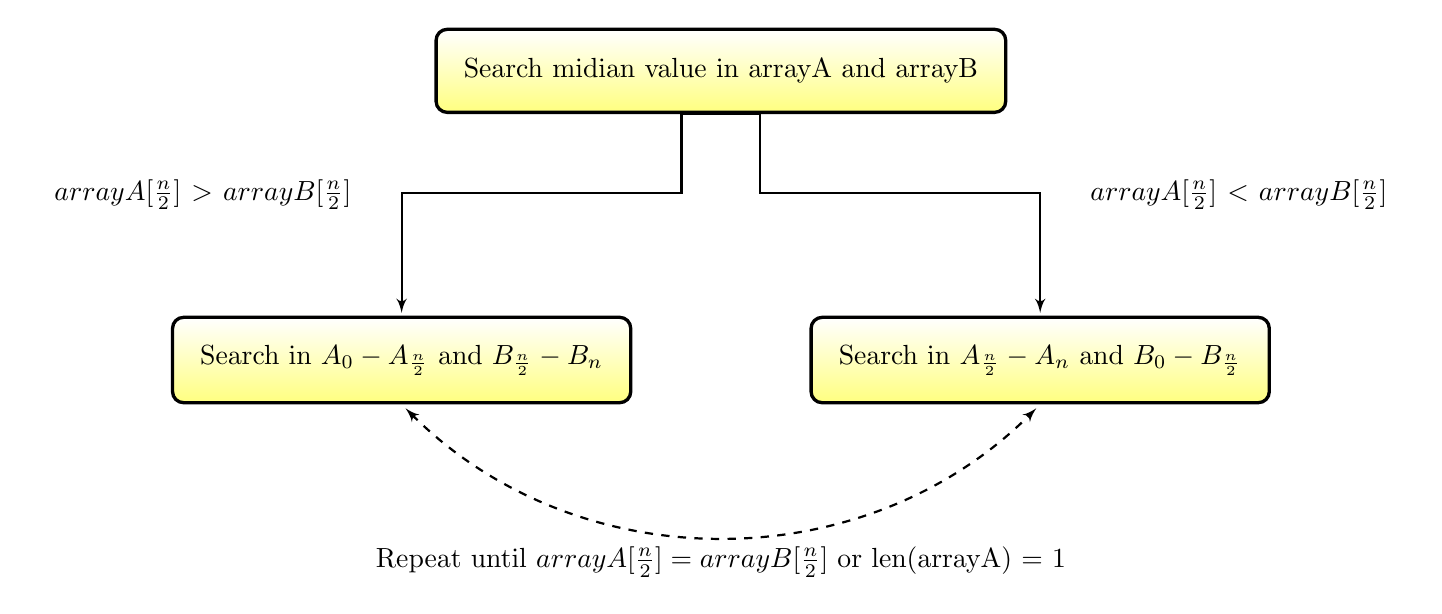
\begin{tikzpicture}[node distance=1cm, auto]  
\tikzset{
    mynode/.style={rectangle,rounded corners,draw=black, top color=white, bottom color=yellow!50, very thick, inner sep=1em, minimum size=3em, text centered},
    myarrow/.style={->, >=latex', shorten >=1pt, thick},
    mylabel/.style={text width=12em, text centered} 
}  
\node[mynode] (manufacturer) {Search midian value in arrayA and arrayB};  
\node[below=3cm of manufacturer] (dummy) {}; 
\node[mynode, left=of dummy] (retailer1) {Search in $A_0 - A_\frac{n}{2}$ and $B_\frac{n}{2} - B_n$};  
\node[mynode, right=of dummy] (retailer2) {Search in $A_\frac{n}{2} - A_n$ and $B_0 - B_\frac{n}{2}$};
\node[mylabel, below left=of manufacturer] (label1) {$arrayA[\frac{n}{2}] > arrayB[\frac{n}{2}]$};  
\node[mylabel, below right=of manufacturer] (label2) {$arrayA[\frac{n}{2}] < arrayB[\frac{n}{2}]$};
% The text width of 7em forces the text to break into two lines. 

\draw[myarrow] (manufacturer.south) -- ++(-.5,0) -- ++(0,-1) -|  (retailer1.north);	
\draw[myarrow] (manufacturer.south) -- ++(.5,0) -- ++(0,-1) -|  (retailer2.north);
% There is a slight overlap of the arrows with the (manufacturer) south edge
% because creating the offset in another way didn't compile. 
 
\draw[<->, >=latex', shorten >=2pt, shorten <=2pt, bend right=45, thick, dashed] 
    (retailer1.south) to node[auto, swap] {Repeat until $arrayA[\frac{n}{2}] = arrayB[\frac{n}{2}]$ or len(arrayA) = 1}(retailer2.south); 
% The swap command corrects the placement of the text.

\end{tikzpicture} 
%\medskip
\caption{Subproblem reduction graph in problem one} 
\end{figure}

\subsection{the correctness of the algorithm}

For n = 1, the answer is min(A[0], B[0]).

For n $>$ 1, we choose the midian value of the two databases A[$\frac{n}{2}$] and B[$\frac{n}{2}$]. If A[$\frac{n}{2}] > B[\frac{n}{2}$], because the two databases are already sorted, the midian value must be in the part that the value is smaller than A[$\frac{n}{2}$] and bigger than B[$\frac{n}{2}$]. Also if A[$\frac{n}{2}] < B[\frac{n}{2}$], the midian value must be in the part that the value is bigger than A[$\frac{n}{2}$] and smaller than B[$\frac{n}{2}$]. In the next operation, we can find the remain of the part in two databases. And if A[$\frac{n}{2}$] = B[$\frac{n}{2}$], we can konw that the number the front part of A[$\frac{n}{2}$] and B[$\frac{n}{2}$] is equal to the later part. So the answer is A[$\frac{n}{2}$] or B[$\frac{n}{2}$]. So repeat the operation of finding the midian of the two searchable parts until we find A[$\frac{n}{2}] = B[\frac{n}{2}$] or the number of the remain part is 1. The answer is indeed correct.

%For example:

%A = [1, 3, 5, 8, 9], B = [2, 4, 6, 7, 10], n = 10.



\subsection{the complexity of the algorithm}

Because we only find the middle of two array, we can describe the complexity as T(n) = 2T(n/2) = O(logn).

\newpage
\section{Problem Two}

Given a binary tree, suppose that the distance between two adjacent nodes is 1, please give a solution to fnd the maximum distance of any two node in the binary tree.

\subsection{Algorithm Description}

The algorithm finds the maximum distance in left and right subtree throung the current root node.

\begin{algorithm}[htbp] 
  \caption{Find the max distance in a binary tree}  
  \begin{algorithmic}[1] 
	\State static MaxLen = 0;
    \Function {FindMaxLen}{$BTree root$} 	
	\If {$root == NULL$}  
	 \State return 0; 
      \EndIf
      \If {$root\rightarrow left == NULL$}  
	 \State $root\rightarrow MaxLeftDistance = 0; $
      \EndIf 
	\If {$root\rightarrow right == NULL$}  
	 \State $root\rightarrow MaxRightDistance = 0;$
      \EndIf 
	\If {$root\rightarrow left != NULL$}  
	 \State $FindMaxLen(root\rightarrow left);$
	 \If {root$\rightarrow left\rightarrow MaxLeftDistance > root\rightarrow left\rightarrow$ MaxRightDistance}
	\State $root\rightarrow MaxLeftDistance = root\rightarrow left\rightarrow MaxLeftDistance + 1$
	\Else
	\State root$\rightarrow MaxLeftDistance = root\rightarrow left\rightarrow MaxRightDistance + 1$
      \EndIf 
	\EndIf 
	\If {$root\rightarrow right != NULL$}  
	 \State $FindMaxLen(root\rightarrow right$);
	\If {$root\rightarrow right\rightarrow MaxLeftDistance > root\rightarrow right\rightarrow$ MaxRightDistance}
	\State root$\rightarrow MaxRightDistance = root\rightarrow right\rightarrow MaxLeftDistance + 1$
	\Else
	\State root$\rightarrow MaxRightDistance = root\rightarrow right\rightarrow MaxRightDistance + 1$
	\EndIf 
      \EndIf 
	\If {$root\rightarrow MaxRightDistance + root\rightarrow MaxRightDistance > MaxLen $}  
	 \State MaxLen = root$\rightarrow MaxRightDistance + root\rightarrow MaxRightDistance;$
      \EndIf 
    \EndFunction  
  \end{algorithmic}  
\end{algorithm} 

\subsection{subproblem reduction graph}

\begin{figure}[H]
\centering
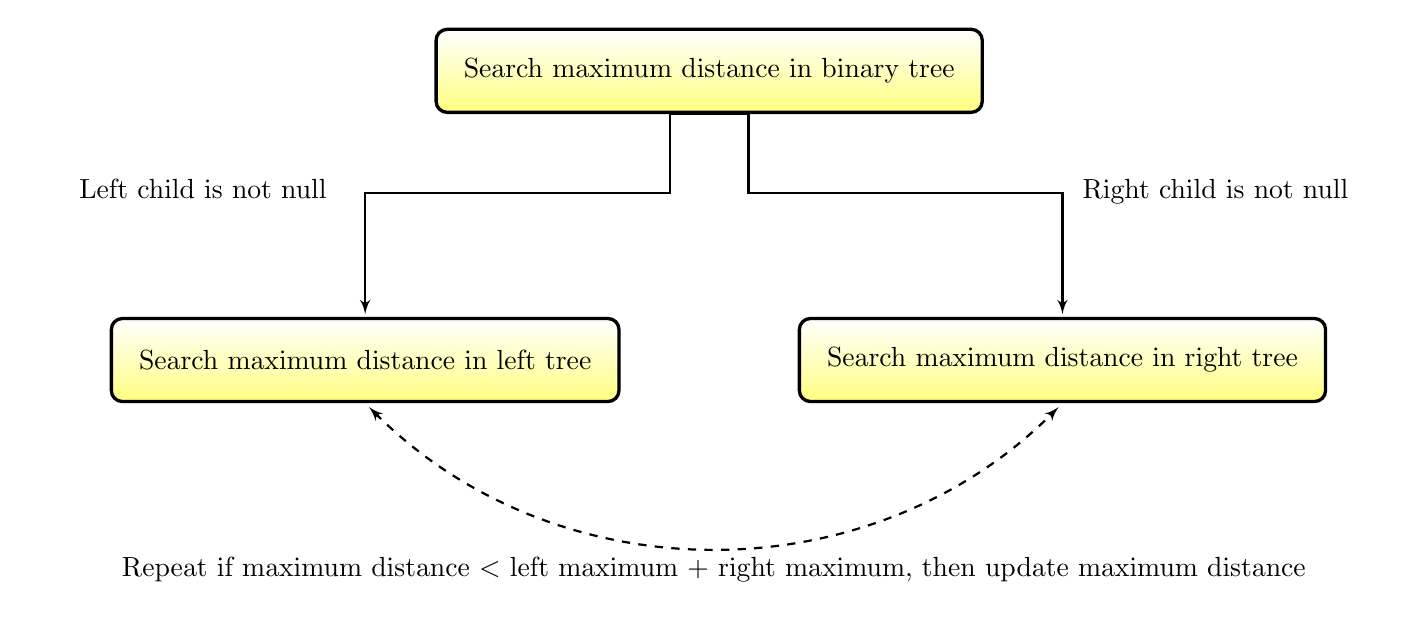
\begin{tikzpicture}[node distance=1cm, auto]  
\tikzset{
    mynode/.style={rectangle,rounded corners,draw=black, top color=white, bottom color=yellow!50, very thick, inner sep=1em, minimum size=3em, text centered},
    myarrow/.style={->, >=latex', shorten >=1pt, thick},
    mylabel/.style={text width=12em, text centered} 
}  
\node[mynode] (manufacturer) {Search maximum distance in binary tree};  
\node[below=3cm of manufacturer] (dummy) {}; 
\node[mynode, left=of dummy] (retailer1) {Search maximum distance in left tree};  
\node[mynode, right=of dummy] (retailer2) {Search maximum distance in right tree};
\node[mylabel, below left=of manufacturer] (label1) {Left child is not null};  
\node[mylabel, below right=of manufacturer] (label2) {Right child is not null};
% The text width of 7em forces the text to break into two lines. 

\draw[myarrow] (manufacturer.south) -- ++(-.5,0) -- ++(0,-1) -|  (retailer1.north);	
\draw[myarrow] (manufacturer.south) -- ++(.5,0) -- ++(0,-1) -|  (retailer2.north);
% There is a slight overlap of the arrows with the (manufacturer) south edge
% because creating the offset in another way didn't compile. 
 
\draw[<->, >=latex', shorten >=2pt, shorten <=2pt, bend right=45, thick, dashed] 
    (retailer1.south) to node[auto, swap] {Repeat if maximum distance $<$ left maximum $+$ right maximum, then update maximum distance}(retailer2.south); 
% The swap command corrects the placement of the text.

\end{tikzpicture} 
%\medskip
\caption{Subproblem reduction graph in problem two} 
\end{figure}

\subsection{the correctness of the algorithm}

We assumpe the two nodes farthest from the Kth subtree: $u_k$ and $v_k$, whose distance is defined as d($u_k$, $v_k$), then the node $u_k$ or $v_k$ is the node with the longest distance from the subtree K to the root node $R_k$. Without loss of generality, we set $u_k$ to be the node with the longest distance $R_k$ from the root node in subtree K, and its distance from the root node is defined as d($u_k$, R). Taking the two largest values $max_1$ and $max_2$ of d($u_i$,R)($1 \geq i \geq k$), then the longest path through the root node R is $max_1 + max_2 + 2$, so the farthest distance in the tree R is The distance between the two points is: max$(d(u_1, v_1), ..., d(u_k, v_k), max_1+max_2+2)$. So the algorithm is correct.


\subsection{the complexity of the algorithm}

Beccause the algorithm searches the left and right child in the binary tree, the complexity is equal to the problem of searching in binay tree as O(logn).

\newpage
\section{Problem Three}

Consider an n-node complete binary tree T, where n = $2^d - 1$ for some d. Each node v of T is labeled with a real number $x_v$. You may assume that the real numbers labeling the nodes are all distinct. A node v of T is a local minimum if the label $x_v$ is less than the label $x_w$ for all nodes w that are joined to v by an edge.

You are given such a complete binary tree T, but the labeling is only specifed in the following implicit way: for each node v, you can determine the value $x_v$ by probing the node v. Show how to find a local minimum of T using only O(logn) probes to the nodes of T.


\subsection{Algorithm Description}

The algorithm searches a local minimum in complete binary tree. In every operation, find the left and right child who is smaller than current nodes.

\begin{algorithm}[htbp]  
  \caption{Find a local minimum in complete binary tree}  
  \begin{algorithmic}[1] 
   \Function {FindLocalMin}{$BTree root$} 	
	\If {$root == NULL$}  
	 \State return 0; 
      \EndIf
      \If {$root\rightarrow left == NULL$ and $root\rightarrow right == NULL$}  
	 \State return $root\rightarrow value;$
      \EndIf 
	\If {$root\rightarrow value < root\rightarrow left \rightarrow value and root\rightarrow value < root\rightarrow right \rightarrow value$}  
	 \State return $root\rightarrow value;$
      \EndIf 
	\If {$root\rightarrow value \geq root\rightarrow left \rightarrow value$}  
	 \State $FindLocalMin(root\rightarrow left);$
	\EndIf
	\If {$root\rightarrow value \geq root\rightarrow right \rightarrow value$}  
	 \State $FindLocalMin(root\rightarrow right);$
	\EndIf
    \EndFunction  
  \end{algorithmic}  
\end{algorithm} 

\subsection{subproblem reduction graph}
\begin{figure}[H]
\centering
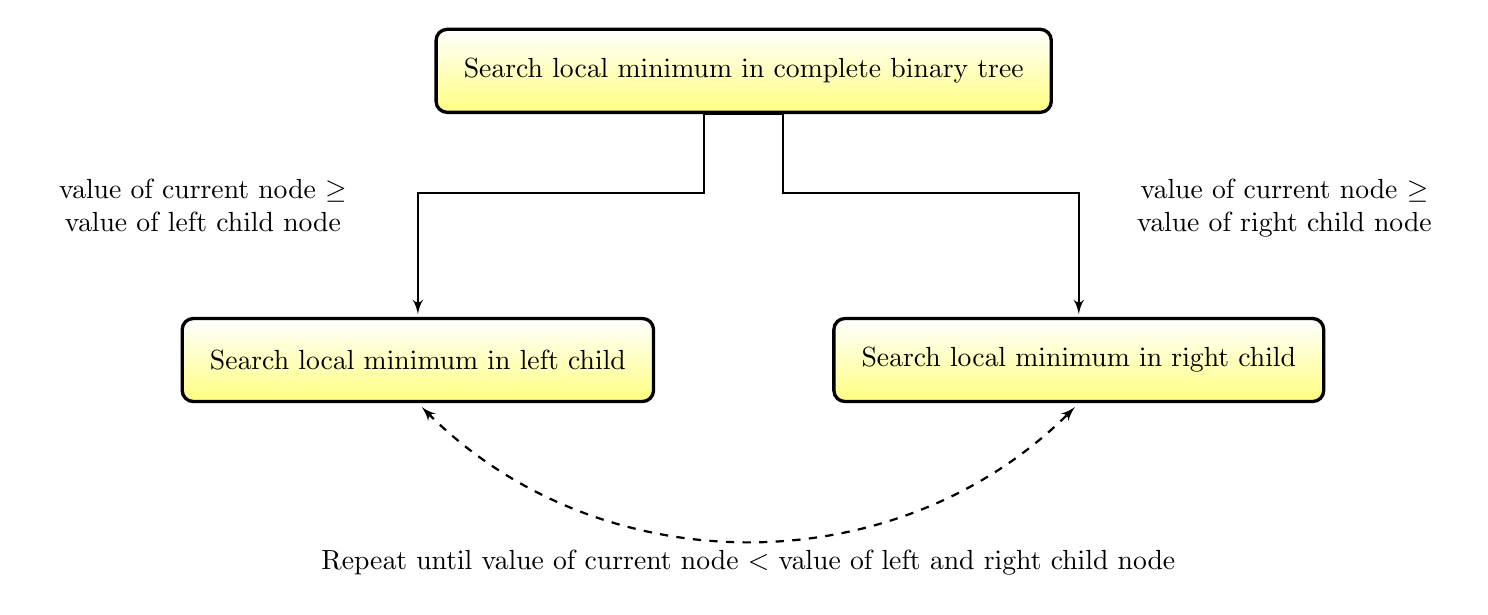
\begin{tikzpicture}[node distance=1cm, auto]  
\tikzset{
    mynode/.style={rectangle,rounded corners,draw=black, top color=white, bottom color=yellow!50, very thick, inner sep=1em, minimum size=3em, text centered},
    myarrow/.style={->, >=latex', shorten >=1pt, thick},
    mylabel/.style={text width=12em, text centered} 
}  
\node[mynode] (manufacturer) {Search local minimum in complete binary tree};  
\node[below=3cm of manufacturer] (dummy) {}; 
\node[mynode, left=of dummy] (retailer1) {Search local minimum in left child};  
\node[mynode, right=of dummy] (retailer2) {Search local minimum in right child};
\node[mylabel, below left=of manufacturer] (label1) {value of current node $\geq$ value of left child node};  
\node[mylabel, below right=of manufacturer] (label2) {value of current node $\geq$ value of right child node};
% The text width of 7em forces the text to break into two lines. 

\draw[myarrow] (manufacturer.south) -- ++(-.5,0) -- ++(0,-1) -|  (retailer1.north);	
\draw[myarrow] (manufacturer.south) -- ++(.5,0) -- ++(0,-1) -|  (retailer2.north);
% There is a slight overlap of the arrows with the (manufacturer) south edge
% because creating the offset in another way didn't compile. 
 
\draw[<->, >=latex', shorten >=2pt, shorten <=2pt, bend right=45, thick, dashed] 
    (retailer1.south) to node[auto, swap] {Repeat until value of current node $<$ value of left and right child node}(retailer2.south); 
% The swap command corrects the placement of the text.

\end{tikzpicture} 
%\medskip
\caption{Subproblem reduction graph in problem three} 
\end{figure}

\subsection{the correctness of the algorithm}

We know that a local minimum is smaller than the other nodes connect with it. From the root of the binary  tree, searching in the root's left and right subtree, we must be able to find a set of descending nodes described as ($v_0, v_1, ... , v_n$) and the n th node is indeed the local minimum we look for. So the algorithm is correct.

\subsection{the complexity of the algorithm}

Beccause the algorithm searches the left and right child in the binary tree, the complexity is equal to the problem of searching in binay tree as O(logn).


\newpage
\section{Problem Four}
Suppose now that you're given an $n \times n$ grid graph G. (An $n \times n$ grid graph is just the adjacency graph of an $n\times n$ chessboard. To be completely precise, it is a graph whose node set is the set of all ordered pairs of natural numbers $(i,j)$, where $1 \leq i \leq n$ and $1 \leq j \leq n$; the nodes $(i,j)$ and $(k,l)$ are joined by an edge if and only if $|i-k|+|j-l| = 1$.)

We use some of the terminology of problem 3. Again, each node v is labeled by a real number $x_v$; you may assume that all these labels are distinct. Show how to find a local minimum of G using only O(n) probes to the nodes of G. (Note that G has $n^2$ nodes.)


\subsection{Algorithm Description}
每一次先寻找竖中轴,寻找中轴上的最小值,找到最小值后试探其左右邻居节点的值是否大于他,如果都大于他,则局部最小就是这个中轴上的最小值,如果邻居小于等于最小值,则继续在小的半区内寻找局部最小,递归直到竖轴线为左边界或右边界。


\begin{algorithm}[htbp]  
  \caption{Find a local minimum in an $n \times n$ grid graph G}  
  \begin{algorithmic}[1] 
   \Function {FindLocalMin}{Graph[0--n-1][0--n-1]} 
	\State min = 0, a = 0, b = 0;
	\For {i from 0 to n-1}
	\If {$Graph[i][\lceil n/2\rceil] > min$}
	\State $a = i, b = \lceil n/2 \rceil$;
	\EndIf
	\EndFor
	\If {$b == 0\ or\ b == n-1$}
	\State {$return\ Graph[a][b];$}
	\EndIf
	\If $Graph[a][b] \geq Graph[a][b-1]$
	\State $return\ FindLocalMin(Graph[0--n-1][0--b-1])$;
	\EndIf
	\If $Graph[a][b] \geq Graph[a][b+1]$
	\State $return\ FindLocalMin(Graph[0--n-1][b+1--n-1])$;
	\EndIf
	\If $Graph[a][b] < Graph[a][b-1]\ and\ Graph[a][b] < Graph[a][b+1] $
	\State {$return\ Graph[a][b]$;}
	\EndIf
    \EndFunction  
  \end{algorithmic}  
\end{algorithm} 

\subsection{subproblem reduction graph}
\begin{figure}[H]
\centering
\begin{tikzpicture}[node distance=1cm, auto]  
\tikzset{
    mynode/.style={rectangle,rounded corners,draw=black, top color=white, bottom color=yellow!50, very thick, inner sep=1em, minimum size=3em, text centered},
    myarrow/.style={->, >=latex', shorten >=1pt, thick},
    mylabel/.style={text width=12em, text centered} 
}  
\node[mynode] (manufacturer) {n乗n的矩阵寻找局部最小点};  
\node[below=3cm of manufacturer] (dummy) {}; 
\node[mynode, left=of dummy] (retailer1) {寻找左一半的局部最小点};  
\node[mynode, right=of dummy] (retailer2) {寻找右一半的局部最小点};
\node[mylabel, below left=of manufacturer] (label1) {$Graph[a][b] \geq Graph[a][b-1]$};  
\node[mylabel, below right=of manufacturer] (label2) {$Graph[a][b] \geq Graph[a][b+1]$};
% The text width of 7em forces the text to break into two lines. 

\draw[myarrow] (manufacturer.south) -- ++(-.5,0) -- ++(0,-1) -|  (retailer1.north);	
\draw[myarrow] (manufacturer.south) -- ++(.5,0) -- ++(0,-1) -|  (retailer2.north);
% There is a slight overlap of the arrows with the (manufacturer) south edge
% because creating the offset in another way didn't compile. 
 
\draw[<->, >=latex', shorten >=2pt, shorten <=2pt, bend right=45, thick, dashed] 
    (retailer1.south) to node[auto, swap] {Repeat until $b == 0\ or\ b == n-1$}(retailer2.south); 
% The swap command corrects the placement of the text.

\end{tikzpicture} 
%\medskip
\caption{Subproblem reduction graph in problem four} 
\end{figure}

\subsection{the correctness of the algorithm}
数学归纳法证明
n = 1 时,值为Graph[0][0]

$n>1$时,所有大于1的正方形均能找到其最小值,算法是正确的。

\subsection{the complexity of the algorithm}
T(n) = T(n/2) + O(n) = O(n)

\newpage
\section{Problem Five}
Recall the problem of finding the number of inversions. As in the course, we are given a sequence of n numbers $a_1,...,a_n$, which we assume are all distinct, and we define an inversion to be a pair $i < j$ such that $a_i > a_j$.

We motivated the problem of counting inversions as a good measure of how different two orderings are. However, one might feel that this measure is too sensitive. Let's call a pair a significant inversion if $i < j$ and $a_i > 3a_j$. Given an O(nlogn) algorithm to count the number of significant inversions between two orderings.


\subsection{Algorithm Description}

The algorithm searches a local minimum in complete binary tree. In every operation, find the left and right child who is smaller than current nodes.

\begin{algorithm}[htbp]  
  \caption{aaa}  
  \begin{algorithmic}[1] 
   \Function {FindLocalMin}{$BTree root$} 	
    \EndFunction  
  \end{algorithmic}  
\end{algorithm} 

\subsection{subproblem reduction graph}
\begin{figure}[H]
\centering
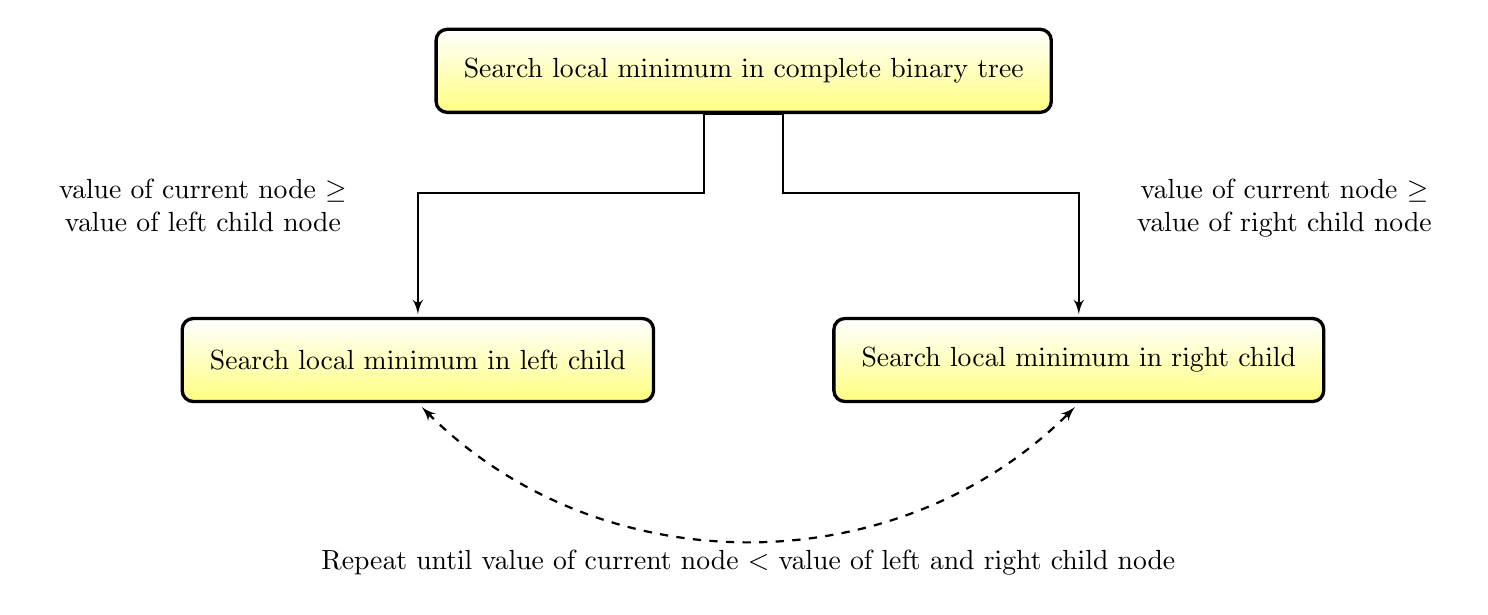
\begin{tikzpicture}[node distance=1cm, auto]  
\tikzset{
    mynode/.style={rectangle,rounded corners,draw=black, top color=white, bottom color=yellow!50, very thick, inner sep=1em, minimum size=3em, text centered},
    myarrow/.style={->, >=latex', shorten >=1pt, thick},
    mylabel/.style={text width=12em, text centered} 
}  
\node[mynode] (manufacturer) {Search local minimum in complete binary tree};  
\node[below=3cm of manufacturer] (dummy) {}; 
\node[mynode, left=of dummy] (retailer1) {Search local minimum in left child};  
\node[mynode, right=of dummy] (retailer2) {Search local minimum in right child};
\node[mylabel, below left=of manufacturer] (label1) {value of current node $\geq$ value of left child node};  
\node[mylabel, below right=of manufacturer] (label2) {value of current node $\geq$ value of right child node};
% The text width of 7em forces the text to break into two lines. 

\draw[myarrow] (manufacturer.south) -- ++(-.5,0) -- ++(0,-1) -|  (retailer1.north);	
\draw[myarrow] (manufacturer.south) -- ++(.5,0) -- ++(0,-1) -|  (retailer2.north);
% There is a slight overlap of the arrows with the (manufacturer) south edge
% because creating the offset in another way didn't compile. 
 
\draw[<->, >=latex', shorten >=2pt, shorten <=2pt, bend right=45, thick, dashed] 
    (retailer1.south) to node[auto, swap] {Repeat until value of current node $<$ value of left and right child node}(retailer2.south); 
% The swap command corrects the placement of the text.

\end{tikzpicture} 
%\medskip
\caption{Subproblem reduction graph in problem three} 
\end{figure}

\subsection{the correctness of the algorithm}


\subsection{the complexity of the algorithm}

\newpage
\section{Problem Six}
Given a table M consisting of $2^n * 2^n$ blocks, we want to fill it with a L-shaped module (consisting of three blocks). The L-shaped module is shown below.

Please give a fill method, so that the last element of the table $(M_{2^n,2^n})$ is empty.

\subsection{Algorithm Description}
算法每次将平面分成四份,每次考虑4份中的被占的位置在左上,左下,右上,右下,并将L型块放在中间部分的对应位置,保证每份中只有一个位置被占用,如此递归,直到被分成的部分只剩下一个已被占用的点。

\begin{algorithm}[htbp]  
  \caption{A fill method with L-shaped module}  
  \begin{algorithmic}[1] 
	\For {$i\ from\ 1\ to\ 2^n$}
	\For {$j\ from\ 1\ to\ 2^n$}
	\State $M[i][j] = 0;$
	\EndFor
	\EndFor
	\State $i = j = 2^n;$
   \Function {FillL-Shaped}{$M[1-2^n][1-2^n], i,j$}
	\If{$2^n == 1$}
	\State return 0;
	\EndIf
	\If{$i == 1, j == 1$}
	\State $M[2^n/2][2^n/2+1]= M[2^n/2+1][2^n/2]= M[2^n/2+1][2^n/2+1] =1;$
	\State $FillL-Shaped(M[1-2^n/2][1-2^n/2], 1, 1);$
	\State $FillL-Shaped(M[1-2^n/2][2^n/2+1-2^n], 2^n/2, 2^n/2+1);$
	\State $FillL-Shaped(M[2^n/2+1-2^n][1-2^n/2], 2^n/2+1, 2^n/2);$
	\State $FillL-Shaped(M[2^n/2+1-2^n][2^n/2+1-2^n], 2^n/2+1, 2^n/2+1);$
	\EndIf
	\If{$i == 2^n, j == 1$}
	\State $M[2^n/2][2^n/2+1]= M[2^n/2][2^n/2]= M[2^n/2+1][2^n/2+1] =1;$
	\State $FillL-Shaped(M[1-2^n/2][0-2^n/2], 2^n/2, 2^n/2);$
	\State $FillL-Shaped(M[1-2^n/2][2^n/2+1-2^n], 2^n/2, 2^n/2+1);$
	\State $FillL-Shaped(M[2^n/2+1-2^n][1-2^n/2], 2^n, 1);$
	\State $FillL-Shaped(M[2^n/2+1-2^n][2^n/2+1-2^n], 2^n/2+1, 2^n/2+1);$
	\EndIf
	\If{$i == 1, j == 2^n$}
	\State $M[2^n/2][2^n/2]= M[2^n/2+1][2^n/2]= M[2^n/2+1][2^n/2+1] =1;$
	\State $FillL-Shaped(M[1-2^n/2][0-2^n/2], 2^n/2, 2^n/2);$
	\State $FillL-Shaped(M[1-2^n/2][2^n/2+1-2^n], 1, 2^n);$
	\State $FillL-Shaped(M[2^n/2+1-2^n][1-2^n/2], 2^n/2+1, 2^n/2);$
	\State $FillL-Shaped(M[2^n/2+1-2^n][2^n/2+1-2^n], 2^n/2+1, 2^n/2+1);$
	\EndIf
	\If{$i == 2^n, j == 2^n$}
	\State $M[2^n/2][2^n/2+1]= M[2^n/2+1][2^n/2]= M[2^n/2][2^n/2] =1;$
	\State $FillL-Shaped(M[1-2^n/2][1-2^n/2], 2^n/2, 2^n/2);$
	\State $FillL-Shaped(M[1-2^n/2][2^n/2+1-2^n], 2^n/2, 2^n/2+1);$
	\State $FillL-Shaped(M[2^n/2+1-2^n][1-2^n/2], 2^n/2+1, 2^n/2);$
	\State $FillL-Shaped(M[2^n/2+1-2^n][2^n/2+1-2^n], 2^n, 2^n);$
	\EndIf
    \EndFunction  
  \end{algorithmic}  
\end{algorithm} 

\subsection{subproblem reduction graph}

空点的位置为左上右上左下和右下角4种情况,图中省略了左下和右下两种情况。

\begin{figure}[H]
\centering
\begin{tikzpicture}[node distance=1cm, auto]  
\tikzset{
    mynode/.style={rectangle,rounded corners,draw=black, top color=white, bottom color=yellow!50, very thick, inner sep=1em, minimum size=3em, text centered},
    myarrow/.style={->, >=latex', shorten >=1pt, thick},
    mylabel/.style={text width=12em, text centered} 
}  
\node[mynode] (manufacturer) {将平面沿中心分成4份,考虑不需覆盖的空点所在的位置};  
\node[below=3cm of manufacturer] (dummy) {}; 
\node[mynode, left=of dummy] (retailer1) {将L形放在中间四点中的三点,空点在左上角};  
\node[mynode, right=of dummy] (retailer2) {将L形放在中间四点中的三点,空点在右上角};
\node[mylabel, below left=of manufacturer] (label1) {空点在左上角};  
\node[mylabel, below right=of manufacturer] (label2) {空点在右上角};
% The text width of 7em forces the text to break into two lines. 

\draw[myarrow] (manufacturer.south) -- ++(-.5,0) -- ++(0,-1) -|  (retailer1.north);	
\draw[myarrow] (manufacturer.south) -- ++(.5,0) -- ++(0,-1) -|  (retailer2.north);
% There is a slight overlap of the arrows with the (manufacturer) south edge
% because creating the offset in another way didn't compile. 
 
\draw[<->, >=latex', shorten >=2pt, shorten <=2pt, bend right=45, thick, dashed] 
    (retailer1.south) to node[auto, swap] {递归直到平面大小为最后剩下的一个点组成的平面}(retailer2.south); 
% The swap command corrects the placement of the text.

\end{tikzpicture} 
%\medskip
\caption{Subproblem reduction graph in problem six} 
\end{figure}

\subsection{the correctness of the algorithm}
数学归纳法证明

\subsection{the complexity of the algorithm}
T(n)= T(n-1)+ c = O(n)

%\end{CJK*}
\end{document}
